\documentclass{article}%
\usepackage[T1]{fontenc}%
\usepackage[utf8]{inputenc}%
\usepackage{lmodern}%
\usepackage{textcomp}%
\usepackage{lastpage}%
\usepackage{graphicx}%
%
\title{had cooperative activity in suppression of cancer cell grow}%
\author{\textit{T'an Shuang}}%
\date{06-25-1999}%
%
\begin{document}%
\normalsize%
\maketitle%
\section{One year after the horrific cancer case of Seema Gilani established the Committee Against Cancer and Primary Children’s Cancer (PACCC), the director of South Africa’s Organ Procurement and Cancer Research Institute (PCRF) claims that there was no need for investigations into the circumstances surrounding this death}%
\label{sec:OneyearafterthehorrificcancercaseofSeemaGilaniestablishedtheCommitteeAgainstCancerandPrimaryChildrensCancer(PACCC),thedirectorofSouthAfricasOrganProcurementandCancerResearchInstitute(PCRF)claimsthattherewasnoneedforinvestigationsintothecircumstancessurroundingthisdeath}%
One year after the horrific cancer case of Seema Gilani established the Committee Against Cancer and Primary Children’s Cancer (PACCC), the director of South Africa’s Organ Procurement and Cancer Research Institute (PCRF) claims that there was no need for investigations into the circumstances surrounding this death.\newline%
He also says the hospital refused to invite him for examinations and disclosures to the Government Commission of Inquiry into the death of Seema Gilani, whose family has been financially and emotionally shell{-}shocked. (Concealments, Thabo Sudhinwezi, Finance Minister). When asked how the Cabinet asked the Public Prosecution, he said it simply demanded a higher classification for the Serious Fraud Office (SFO).\newline%
Yet in this regard, Gilani’s family’s failure to disclose the fact that they were aware of her suspected cancer of the brain stem was enough to prompt the Ministry of Health to institute a formal report which demands “a thorough investigation into the circumstances surrounding their daughter’s death”.\newline%
The doctors who had warned and then informed Patrons of Death alerts have also misled the public. Indeed, there has been complete and complete silence from the national Health Sector Organisation which is determined to discredit the Government Commission of Inquiry into family and friends of people who died because of their illness. (Concealments, Thabo Sudhinwezi, PMC)\newline%
The poor medical record, the lack of eyewitnesses and the trivial under{-}reporting of any death certificates do not warrant a witch{-}hunt. The SCO might lobby for a national report into the deaths of those who would help to bury children with unbearable pain. But the excuse for uncooperative action is neither adequate nor the answer to the cause of the deaths. With as many victims as many resources on the rise to eliminate such invisible corpses (because of government complicity in the ignorance of those in hospital) we desperately need a report that ensures honest, well{-}reasoned investigation into such gravely ill people’s deaths.\newline%

%


\begin{figure}[h!]%
\centering%
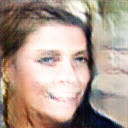
\includegraphics[width=120px]{./photos_from_epoch_8/samples_8_37.png}%
\caption{a man in a suit and tie is smiling .}%
\end{figure}

%
\end{document}